\part{图论}

\chapter{最短路}

\section{单源最短路}
\entrymeta{Dijkstra $O(m\log m)$；Johnson $O(nm\log m)$}
\subsection{P4779 【模板】单源最短路径（标准版）}\label{p4779-ux6a21ux677fux5355ux6e90ux6700ux77edux8defux5f84ux6807ux51c6ux7248}






\begin{codeline}
#define N 100005
class Way {
public:
    int v, w;
};
class State {
public:
    int idx, d;
};
inline bool operator<(const State& A, const State& B) {
    return A.d > B.d;
}
vector<Way> way[N];
int d[N];
priority_queue<State> q;
bool visited[N];
int main() {
    ios::sync_with_stdio(false);
    cin.tie(nullptr);
    int n, m, r;
    memset(d, 0x3f, sizeof(d));
    cin >> n >> m >> r;
    int u, v, w;
    d[r] = 0;
    q.push({r, d[r]});
    while(m-- > 0) {
        cin >> u >> v >> w;
        way[u].push_back({v, w});
    }
    State now;
    while(!q.empty()) {
        now = q.top();
        q.pop();
        if(!visited[now.idx]) {
            visited[now.idx] = true;
            for(Way& e : way[now.idx]) {
                if(d[now.idx] + e.w < d[e.v]) {
                    d[e.v] = d[now.idx] + e.w;
                    q.push({e.v, d[e.v]});
                }
            }
        }
    }
    for(int i = 1; i <= n; i++) {
        cout << (d[i]) << ' ';
    }
\end{codeline}
\vspace{-0.9\baselineskip}
\begin{codeline}[firstnumber=47]
}
\end{codeline}


\subsection{P5905 【模板】全源最短路（Johnson）}\label{p5905-ux6a21ux677fux5168ux6e90ux6700ux77edux8defjohnson}












\begin{codeline}
#define N 3005

class Way {
public:
    int64 v, w;
};
class State {
public:
    int64 idx, d;
};
inline bool operator<(const State& A, const State& B) {
    return A.d > B.d;
}
vector<Way> way[N];
int64 d[N];
int64 h[N];
queue<int64> q;
int64 round_cnt[N];
bool in_queue[N];
priority_queue<State> pq;
bool visited[N];
int main() {
    ios::sync_with_stdio(false);
    cin.tie(nullptr);
    int n, m;
    memset(h, 0x3f, sizeof(h));

    cin >> n >> m;
    int u, v, w;
    while(m-- > 0) {
        cin >> u >> v >> w;
        way[u].push_back({v, w});
    }
    for(int i = 1; i <= n; i++) {
        way[0].push_back({i, 0});
    }
    int64 idx;
    h[0] = 0;
    q.push(0);
    bool negative_circle = false;
    while(!q.empty() && !negative_circle) {
        idx = q.front();
        q.pop();
        in_queue[idx] = false;
        for(Way& e : way[idx]) {
            if(h[idx] + e.w < h[e.v]) {
\end{codeline}
\vspace{-0.9\baselineskip}
\begin{codeline}[firstnumber=47]
                if(round_cnt[e.v] > n) {
                    negative_circle = true;
                    break;
                } else {
                    h[e.v] = h[idx] + e.w;
                    if(!in_queue[e.v]) {
                        round_cnt[e.v]++;
                        q.push(e.v);
                        in_queue[e.v] = true;
                    }
                }
            }
        }
    }

    if(negative_circle) {
        cout << "-1";
        return 0;
    } else {
        for(int i = 1; i <= n; i++) {
            for(Way& e : way[i]) {
                e.w += h[i] - h[e.v];
            }
        }

        int64 sum, tmp;
        for(int i = 1; i <= n; i++) {
            sum = 0;
            memset(d, 0x3f, sizeof(d));
            memset(visited, 0, sizeof(visited));
            State now;
            pq.push({i, 0});
            d[i] = 0;
            while(!pq.empty()) {
                now = pq.top();
                pq.pop();
                if(!visited[now.idx]) {
                    visited[now.idx] = true;
                    for(Way& e : way[now.idx]) {
                        if(d[now.idx] + e.w < d[e.v]) {
                            d[e.v] = d[now.idx] + e.w;
                            pq.push({e.v, d[e.v]});
                        }
                    }
                }
            }
\end{codeline}
\vspace{-0.9\baselineskip}
\begin{codeline}[firstnumber=93]
            for(int j = 1; j <= n; j++) {
                if(d[j] >= (1ll << 31)) {
                    if(i != j) {
                        sum += 1000000000ll * j;
                    }
                } else {
                    if(i != j) {
                        sum += (d[j] + h[j] - h[i]) * j;
                    }
                }
            }
            cout << (sum) << '\n';
        }
    }
}
\end{codeline}


\subsection{P3953 {[}NOIP 2017 提高组{]} 逛公园}\label{p3953-noip-2017-ux63d0ux9ad8ux7ec4-ux901bux516cux56ed}






\begin{codeline}
const int N = 100005;
const int K = 51;
const int INF = 0x3f3f3f3f;
class OriEdge {
public:
    int v, w;
};

class OriNode {
public:
    vector<OriEdge> oe;
    int dfn, low;
    int root;
    bool inStack;
};

class Edge {
public:
    int v, w;
};

class Node {
public:
    vector<Edge> oe;
    int dis;
    int ie;
    long long dp[K];
    bool onzl, visited;
};

OriNode old[N];
Node node[N];

int n, m, k, p;
int dfn = 1;
vector<int> st;

/*
 * 求u可达部分的强连通分量并记录分量编号
 */
void tarjan(int u) {
    old[u].low = old[u].dfn = dfn++;
    old[u].root = u;
    st.push_back(u);
    old[u].inStack = true;
    for(OriEdge& e : old[u].oe) {
\end{codeline}
\vspace{-0.9\baselineskip}
\begin{codeline}[firstnumber=47]
        if(!e.w) {
            if(!old[e.v].dfn) {
                tarjan(e.v);
            }
            if(old[u].low > old[e.v].low && old[e.v].inStack) {
                old[u].low = old[e.v].low;
            }
        }
    }

    if(old[u].low == old[u].dfn) {
        if(st.back() != u) {
            node[u].onzl = true;
        }

        while(st.back() != u) {
            old[st.back()].root = u;
            old[st.back()].inStack = false;
            st.pop_back();
        }
        st.pop_back();
        old[u].inStack = false;
    }
}

class State {
public:
    int u, dis;
    bool operator<(const State& O) const {
        return dis > O.dis;
    }
};

int ptr[N];

int main() {
    ios::sync_with_stdio(false);
    cin.tie(nullptr);
    int T;
    cin >> T;
    while(T--) {
        cin >> n >> m >> k >> p;
        dfn = 1;
        st.clear();
        for(int i = 1; i <= n; i++) {
            old[i] = {{}, 0, 0, 0, false};
\end{codeline}
\vspace{-0.9\baselineskip}
\begin{codeline}[firstnumber=93]
            node[i] = {{}, INF, 0};
            for(int j = 0; j <= k; j++) {
                node[i].dp[j] = 0;
            }
            node[i].onzl = false;
            node[i].visited = false;
        }
        int u, v, w;
        for(int i = 1; i <= m; i++) {
            cin >> u >> v >> w;
            old[u].oe.push_back({v, w});
        }

        for(int i = 1; i <= n; i++) {
            if(!old[i].dfn) {
                tarjan(i);
            }
        }

        long long ans;
        {
            for(u = 1; u <= n; u++) {
                for(OriEdge& e : old[u].oe) {
                    int nu = old[u].root;
                    int nv = old[e.v].root;
                    if(nu != nv) {
                        node[nu].oe.push_back({nv, e.w});
                    }
                }
            }

            node[1].dis = 0;
            priority_queue<State> q;
            q.push({1, 0});
            State cur;
            while(!q.empty()) {
                cur = q.top();
                q.pop();
                if(node[cur.u].visited) {
                    continue;
                } else {
                    node[cur.u].visited = true;
                }
                for(Edge& e : node[cur.u].oe) {
                    int dis = node[cur.u].dis + e.w;
                    if(node[e.v].dis > dis) {
\end{codeline}
\vspace{-0.9\baselineskip}
\begin{codeline}[firstnumber=139]
                        node[e.v].dis = dis;
                        node[e.v].ie = 1;
                        q.push({e.v, dis});
                    } else if(node[e.v].dis == dis) {
                        node[e.v].ie++;
                    }
                }
            }
            queue<int> topo;
            for(int i = 1; i <= n; i++) {
                if(node[i].visited) {
                    if(node[i].onzl) {
                        node[i].dp[0] = -1;
                    }
                    if(!node[i].ie) {
                        topo.push(i);
                    }
                }
            }

            int tidx = 1;
            while(!topo.empty()) {
                u = topo.front();
                topo.pop();
                ptr[tidx++] = u;
                for(Edge& e : node[u].oe) {
                    if(node[u].dis + e.w - node[e.v].dis == 0) {
                        node[e.v].ie--;
                        if(!node[e.v].ie) {
                            topo.push(e.v);
                        }
                    }
                }
            }

            if(!node[1].onzl) {
                node[1].dp[0] = 1;
            }
            for(int i = 0; i <= k; i++) {
                for(int j = 1; j < tidx; j++) {
                    u = ptr[j];
                    for(Edge& e : node[u].oe) {
                        if(node[e.v].dp[i] != -1) {
                            int g = node[u].dis + e.w - node[e.v].dis;
                            if(i + g <= k) {
                                if(node[u].dp[i] == -1) {
\end{codeline}
\vspace{-0.9\baselineskip}
\begin{codeline}[firstnumber=185]
                                    node[e.v].dp[i + g] = -1;
                                } else {
                                    node[e.v].dp[i + g] += node[u].dp[i];
                                    node[e.v].dp[i + g] %= p;
                                }
                            }
                        }
                    }
                }
            }

            ans = 0;
            int root_n = old[n].root;
            for(int i = 0; i <= k; i++) {
                if(node[root_n].dp[i] == -1) {
                    ans = -1;
                    break;
                } else {
                    ans += node[root_n].dp[i];
                    ans %= p;
                }
            }
        }
        cout << (ans) << '\n';
    }
}
\end{codeline}
\begin{warnbox}
Johnson 先跑 SPFA 求势能，再对每个源跑 Dijkstra；判不可达直接与 INF 比较。
\end{warnbox}

\section{差分约束}
\entrymeta{$O(nm)$}
\subsection{P5960 【模板】差分约束}\label{p5960-ux6a21ux677fux5deeux5206ux7ea6ux675f}






\begin{codeline}
#define N 5005
class Edge {
public:
    int v, l;
};
int n, m;
int ie[N];
vector<Edge> oe[N];
int dist[N];
int io_cnt[N];
bool in_queue[N];
int main() {
    ios::sync_with_stdio(false);
    cin.tie(nullptr);
    cin >> n >> m;
    int u, v, l;
    while(m-- > 0) {
        cin >> v >> u >> l;
        ie[v]++;
        oe[u].push_back({v, l});
    }

    for(int i = 1; i <= n; i++) {
        ie[i]++;
        oe[0].push_back({i, 0});
    }

    memset(dist, 0x3f, sizeof(int) * (n + 1));
    dist[0] = 0;
    queue<int> q;
    q.push(0);
    int temp;
    bool negative_circle = false;
    in_queue[0] = true;
    while(!q.empty()) {
        temp = q.front();
        q.pop();
        io_cnt[temp]++;
        in_queue[temp] = false;
        if(io_cnt[temp] > n) {
            negative_circle = true;
            break;
        }
        for(Edge& e : oe[temp]) {

            if(dist[temp] + e.l < dist[e.v]) {
\end{codeline}
\vspace{-0.9\baselineskip}
\begin{codeline}[firstnumber=47]
                dist[e.v] = dist[temp] + e.l;
                if(!in_queue[e.v]) {
                    in_queue[e.v] = true;
                    q.push(e.v);
                }
            }
        }
    }
    if(!negative_circle) {
        for(int i = 1; i <= n; i++) {
            cout << (dist[i]) << ' ';
        }
    } else {
        cout << "NO";
    }
}
\end{codeline}
\begin{warnbox}
最长路/最短路方向与不等式符号要统一；有负环则无解。
\end{warnbox}


\chapter{树上问题}

\section{LCA}
\entrymeta{$O(\log n)$}
\begin{codeline}
/*
 * 返回x、y的最近公共祖先
 */
int getLCA(int x, int y) {
    if(node[x].d < node[y].d) {
        swap(x, y);
    }
    for(int i = LOGN - 1; i >= 0 && node[x].d > node[y].d; i--) {
        if(node[x].d >= node[y].d + (1 << i)) {
            x = node[x].fa[i];
        }
    }
    if(x == y) {
        return x;
    } else {
        for(int i = LOGN - 1; i >= 0; i--) {
            if(node[x].fa[i] != node[y].fa[i]) {
                x = node[x].fa[i];
                y = node[y].fa[i];
            }
        }
        return node[x].fa[0];
    }
}

/*
 * 根据fa[0]预处理倍增祖先，深度在调用前填好
 */
void init() {
    for(int i = 1; i < LOGN; i++) {
        for(int j = 1; j <= n; j++) {
            node[j].fa[i] = node[node[j].fa[i - 1]].fa[i - 1];
        }
    }
}
\end{codeline}
\begin{warnbox}
倍增表 \texttt{LOGN} 要满足 \texttt{2\textasciicircum{}LOGN \textgreater{} n}。
\end{warnbox}

\section{直径}
\entrymeta{$O(n)$}
\subsection{P3304 {[}SDOI2013{]} 直径}\label{p3304-sdoi2013-ux76f4ux5f84}


\begin{codeline}
#define N 200005
class Edge {
public:
    int64 v, l, cnt;
};

class Node {
public:
    vector<Edge> oe;
    int64 depth;
};

Node node[N];
int64 n;

int64 max_d = 0;
int64 max_len = 0;
int64 s_idx = 0;
int64 le = -1, re = -1;
vector<int64> diameter;

void toOneSide(int64 idx, int64 fa, int64 d) {
    if(d > max_d) {
        s_idx = idx;
        max_d = d;
    }
    for(Edge& e : node[idx].oe) {
        if(e.v != fa) {
            toOneSide(e.v, idx, d + e.l);
        }
    }
}

void getDiameter(int64 idx, int64 fa, int64 d) {
    if(d > max_len && node[idx].oe.size() == 1) {
        max_len = d;
    }
    for(Edge& e : node[idx].oe) {
        if(e.v != fa) {
            getDiameter(e.v, idx, d + e.l);
        }
    }
}

bool getDiameterNode(int64 idx, int64 fa, int64 d) {
    diameter.push_back(idx);
\end{codeline}
\vspace{-0.9\baselineskip}
\begin{codeline}[firstnumber=47]
    if(d == max_len) {
        return true;
    }
    for(Edge& e : node[idx].oe) {
        if(e.v != fa) {
            if(getDiameterNode(e.v, idx, d + e.l)) {
                return true;
            }
        }
    }
    diameter.pop_back();
    return false;
}

bool getMiddle(int64 idx, int64 fa, int64 d, int64 node_idx) {
    if(d * 2 == max_len) {
        le = re = idx;
        return true;
    }
    for(Edge& e : node[idx].oe) {
        if(e.v == diameter[node_idx + 1]) {
            if((d + e.l) * 2 > max_len) {
                le = idx;
                re = e.v;
                return true;
            }
            if(getMiddle(e.v, idx, d + e.l, node_idx + 1)) {
                return true;
            }
        }
    }
    return false;
}

int64 getSharedBranch(int64 idx, int64 fa, int64 d) {
    int64 cnt = 0, cnt_sum = 0;
    if(d == max_len) {
        return 1;
    } else {
        for(Edge& e : node[idx].oe) {
            if(e.v != fa) {
                cnt = getSharedBranch(e.v, idx, d + e.l);
                e.cnt = cnt;
                cnt_sum += cnt;
            }
        }
\end{codeline}
\vspace{-0.9\baselineskip}
\begin{codeline}[firstnumber=93]
        return cnt_sum;
    }
}

int64 getDepth(int64 idx, int64 fa, int64 d) {
    int64 maximum = d;
    node[idx].depth = d;
    for(Edge& e : node[idx].oe) {
        if(e.v != fa) {
            maximum = max(maximum, getDepth(e.v, idx, d + e.l));
        }
    }
    return maximum;
}

int64 getCount(int64 idx, int64 fa, int64 d, int64 td) {
    if(d == td) {
        if(node[idx].oe.size() == 1 && d != 0) {
            return 1;
        } else {
            return 0;
        }
    }
    int64 cnt = 0, cnt_sum = 0;
    for(Edge& e : node[idx].oe) {
        if(e.v != fa) {
            cnt = getCount(e.v, idx, d + e.l, td);
            e.cnt = cnt;
            cnt_sum += cnt;
        }
    }
    return cnt_sum;
}

int64 getSharedNode(int64 idx, int64 fa, int64 tc) {
    int64 res = 0;
    for(Edge& e : node[idx].oe) {
        if(e.v != fa && e.cnt == tc) {
            res += getSharedNode(e.v, idx, tc) + 1;
        }
    }
    return res;
}

int main() {
    ios::sync_with_stdio(false);
\end{codeline}
\vspace{-0.9\baselineskip}
\begin{codeline}[firstnumber=139]
    cin.tie(nullptr);
    cin >> n;

    int64 u, v, l;
    for(int64 i = 1; i < n; i++) {
        cin >> u >> v >> l;
        node[u].oe.push_back({v, l, 0});
        node[v].oe.push_back({u, l, 0});
    }

    toOneSide(1, 0, 0);
    getDiameter(s_idx, 0, 0);
    getDiameterNode(s_idx, 0, 0);
    getMiddle(s_idx, 0, 0, 0);

    int64 l_max, r_max, l_cnt, r_cnt, l_share, r_share, middle;
    int64 e_cnt = 0;

    if(le == re) {
        middle = le;
        l_max = getDepth(le, re, 0);
        l_cnt = getCount(le, re, 0, l_max);

        int64 branch_cnt = node[middle].oe.size();
        for(Edge& e : node[middle].oe) {
            if(e.cnt != 0) {
                branch_cnt--;
                le = e.v;
            }
        }
        re = middle;

        if(branch_cnt != 2) {
            cout << (max_len) << '\n'
                 << (0ll) << '\n';
        } else {
            e_cnt = getSharedNode(le, 0, l_cnt);
        }
    }

    l_max = getDepth(le, re, 0);
    r_max = getDepth(re, le, 0);
    l_cnt = getCount(le, re, 0, l_max);
    r_cnt = getCount(re, le, 0, r_max);

    l_share = 0;
\end{codeline}
\vspace{-0.9\baselineskip}
\begin{codeline}[firstnumber=185]
    r_share = 0;
    l_share = getSharedNode(le, re, l_cnt);
    r_share = getSharedNode(re, le, r_cnt);
    e_cnt = l_share + r_share + 1;
    cout << (max_len) << '\n'
         << (e_cnt) << '\n';
}
\end{codeline}


\subsection{B4016 树的直径}\label{b4016-ux6811ux7684ux76f4ux5f84}


\begin{codeline}
const int N = 100005;
const int INF = 0x3f3f3f3f;

class Node {
public:
    vector<int> oe;
    int w, longest;
};

class Graph {
public:
    Node node[N];
    int d_s, d_t, d_l;
    int core;
    int node_cnt;
    vector<int> trace;

    void d_dfs1(int cur, int fa, int d) {
        if(d > d_l) {
            d_s = cur;
            d_l = d;
        }
        for(int son : node[cur].oe) {
            if(son != fa) {
                d_dfs1(son, cur, d + 1);
            }
        }
    }

    int d_dfs2(int cur, int fa) {
        int w;
        for(int i = 0; i < node[cur].oe.size(); i++) {
            int son = node[cur].oe[i];
            if(son != fa) {
                w = d_dfs2(son, cur);
                if(w > node[cur].w) {
                    node[cur].w = w;
                    node[cur].longest = son;
                }
            }
        }
        node[cur].w++;
        return node[cur].w;
    }

    void d_dfs3(int cur, int fa, int& k) {
\end{codeline}
\vspace{-0.9\baselineskip}
\begin{codeline}[firstnumber=47]
        trace.push_back(cur);
        for(int i = 0; i < node[cur].oe.size() && k; i++) {
            int son = node[cur].oe[i];
            if(son != fa) {
                k--;
                d_dfs3(son, cur, k);
                trace.push_back(cur);
            }
        }
    }

    void get_diameter(int start = 1) {
        d_dfs1(start, 0, 1);
        d_l = d_dfs2(d_s, 0);
    }

    void add_edge(int u, int v) {
        node[u].oe.push_back(v);
        node[v].oe.push_back(u);
    }

    void init(int size) {
        node_cnt = size;
        for(int i = 0; i <= node_cnt; i++) {
            node[i].oe.clear();
            node[i].w = 0;
            node[i].longest = -1;
        }
        trace.clear();
        d_s = 0;
        d_t = 0;
        d_l = 0;
    }

    void solve() {
        get_diameter();
        cout << (d_l - 1) << '\n';
    }
};

Graph graph;

int main() {
    ios::sync_with_stdio(false);
    cin.tie(nullptr);
    int n, u, v;
\end{codeline}
\vspace{-0.9\baselineskip}
\begin{codeline}[firstnumber=93]
    cin >> n;
    graph.init(n);
    for(int i = 1; i < n; i++) {
        cin >> u >> v;
        graph.add_edge(u, v);
    }

    graph.solve();
}
\end{codeline}
\begin{warnbox}
两次 DFS 只适用于非负边权；带负权要用树形 DP。
\end{warnbox}

\section{偏心距}
\entrymeta{$O(n)$}
\subsection{P1099 {[}NOIP 2007 提高组{]} 树网的核}\label{p1099-noip-2007-ux63d0ux9ad8ux7ec4-ux6811ux7f51ux7684ux6838}






\begin{codeline}
const int N = 305;
int n, s;

class Edge {
public:
    int v;
    int l;
};

class Node {
public:
    int dis;
    bool on_diameter;
    vector<Edge> oe;
};

Node node[N];

vector<Edge> path;
vector<Edge> temp;
int max_d = 0, start;

void dfs1(int u, int fa, int d) {
    if(d > max_d) {
        start = u;
        max_d = d;
    }

    for(Edge& e : node[u].oe) {
        if(e.v != fa) {
            dfs1(e.v, u, d + e.l);
        }
    }
}

void dfs2(int u, int fa, int d) {
    if(d > max_d) {
        max_d = d;
        if(node[u].oe.size() <= 1) {
            path.assign(temp.begin(), temp.end());
        }
    }

    for(Edge& e : node[u].oe) {
        if(e.v != fa) {
            temp.push_back(e);
\end{codeline}
\vspace{-0.9\baselineskip}
\begin{codeline}[firstnumber=47]
            dfs2(e.v, u, d + e.l);
            temp.pop_back();
        }
    }
}

int dfs3(int u, int fa) {
    for(Edge& e : node[u].oe) {
        if(e.v != fa) {
            node[u].dis = max(node[u].dis, dfs3(e.v, u) + e.l);
        }
    }
    return node[u].dis;
}

int main() {
    ios::sync_with_stdio(false);
    cin.tie(nullptr);
    cin >> n >> s;
    int u, v, l;
    for(int i = 1; i < n; i++) {
        cin >> u >> v >> l;
        node[u].oe.push_back({v, l});
        node[v].oe.push_back({u, l});
    }

    max_d = -2147483648;
    dfs1(1, 0, 0);
    max_d = -2147483648;
    temp.push_back({start, 0});
    dfs2(start, 0, 0);

    int d = 0, cnt = 0;
    int middle = 0;
    int head, tail;
    for(int i = 0; i < path.size(); i++) {
        Edge& e = path[i];
        if((d + e.l) > max_d / 2) {
            if(max_d / 2 - d >= d + e.l - max_d / 2) {
                middle = i;
            } else {
                middle = i - 1;
            }
            break;
        }
        d += e.l;
\end{codeline}
\vspace{-0.9\baselineskip}
\begin{codeline}[firstnumber=93]
    }

    for(int i = 0; i < path.size(); i++) {
        Edge& e = path[i];
        node[e.v].on_diameter = true;
    }

    dfs3(path[middle].v, 0);

    int min_bias = 2147483647;
    int bias;
    bool is_legal;

    for(int i = 0; i <= middle; i++) {
        d = 0;
        bias = 0;
        is_legal = false;
        if(i > 0) {
            bias = max(bias, node[path[i - 1].v].dis + path[i].l);
        }
        for(int j = i; j < path.size(); j++) {
            if(i != j) {
                d += path[j].l;
            }
            if(d > s) {
                bias = max(bias, node[path[j].v].dis + path[j].l);
                break;
            }
            if(j == middle) {
                is_legal = true;
            }
            for(Edge& e : node[path[j].v].oe) {
                if(!node[e.v].on_diameter) {
                    bias = max(bias, node[e.v].dis + e.l);
                }
            }
        }
        if(is_legal) {
            min_bias = min(min_bias, bias);
        }
    }

    cout << (min_bias);
}
\end{codeline}
\begin{warnbox}
单调队列维护直径上的最优区间。
\end{warnbox}

\section{树链剖分}
\entrymeta{$O(\log^2 n)$}
\subsection{P3384 【模板】重链剖分/树链剖分}\label{p3384-ux6a21ux677fux91cdux94feux5256ux5206ux6811ux94feux5256ux5206}


\begin{codeline}
class HLD {
public:
    class Node {
    public:
        vector<int64> oe;
        int64 fa, d, w;
        int64 heavy, dfn, link_head;
    };

    vector<Node> node;
    int64 root = 1;
    int64 dfncnt = 0;

    /*
     * 初始化 n 个点的空树，注意初始化半群结构
     */
    void init(int64 n) {
        node.assign(n + 1, Node());
        root = 1;
        dfncnt = 0;
    }

    /*
     * 添加无向边
     */
    void add_edge(int64 u, int64 v) {
        node[u].oe.push_back(v);
        node[v].oe.push_back(u);
    }

    void dfs1(int u, int fa) {
        node[u].fa = fa;
        node[u].d = node[fa].d + 1;
        node[u].w = 1;
        node[u].heavy = 0;
        int best = 0;
        for(int v : node[u].oe) {
            if(v != fa) {
                dfs1(v, u);
                node[u].w += node[v].w;
                if(node[v].w > best) {
                    best = node[v].w;
                    node[u].heavy = v;
                }
            }
        }
\end{codeline}
\vspace{-0.9\baselineskip}
\begin{codeline}[firstnumber=47]
    }

    void dfs2(int u, int h) {
        node[u].dfn = ++dfncnt;
        node[u].link_head = h;
        if(node[u].heavy) {
            dfs2(node[u].heavy, h);
        }
        for(int v : node[u].oe) {
            if(v != node[u].fa && v != node[u].heavy) {
                dfs2(v, v);
            }
        }
    }

    /*
     * 以 u 为根建立树链剖分
     */
    void build(int64 u) {
        root = u;
        dfncnt = 0;
        dfs1(root, 0);
        dfs2(root, root);
    }

    /*
     * 求 u、v 的最近公共祖先
     */
    int64 lca(int64 u, int64 v) {
        while(node[u].link_head != node[v].link_head) {
            if(node[node[u].link_head].d < node[node[v].link_head].d) {
                swap(u, v);
            }
            u = node[node[u].link_head].fa;
        }
        return node[u].d < node[v].d ? u : v;
    }

    /*
     * 对 dfn 区间 [l, r] 施加修改 x；在这里接入题目需要的半群
     */
    void dfnmod(int l, int r, int x) {
    }

    /*
     * 查询 dfn 区间 [l, r]，x 为题目需要的查询参数
\end{codeline}
\vspace{-0.9\baselineskip}
\begin{codeline}[firstnumber=93]
     */
    int64 dfnquery(int l, int r) {
        return 0;
    }

    /*
     * 将 u 到 v 路径上的点权加 x
     */
    void add(int u, int v, int x) {
        while(node[u].link_head != node[v].link_head) {
            if(node[node[u].link_head].d < node[node[v].link_head].d) {
                swap(u, v);
            }
            dfnmod(node[node[u].link_head].dfn, node[u].dfn, x);
            u = node[node[u].link_head].fa;
        }
        if(node[u].d > node[v].d) {
            swap(u, v);
        }
        dfnmod(node[u].dfn, node[v].dfn, x);
    }

    /*
     * 查询 u 到 v 路径上的信息，x 为题目需要的查询参数
     */
    int query(int u, int v) {
        int res = 0;
        while(node[u].link_head != node[v].link_head) {
            if(node[node[u].link_head].d < node[node[v].link_head].d) {
                swap(u, v);
            }
            res += dfnquery(node[node[u].link_head].dfn, node[u].dfn);
            u = node[node[u].link_head].fa;
        }
        if(node[u].d > node[v].d) {
            swap(u, v);
        }
        res += dfnquery(node[u].dfn, node[v].dfn);
        return res;
    }
};
\end{codeline}


\subsection{P4069 {[}SDOI2016{]} 游戏}\label{p4069-sdoi2016-ux6e38ux620f}


\begin{codeline}
const int64 INF = 0x3f3f3f3f3f3f3f3f;
const int64 INIT_VALUE = 123456789123456789;
const int64 N = 100005;

class Edge {
public:
    int64 v, l;
};

class HLDTreeNode {
public:
    vector<Edge> oe;                     // 边，含指向父节点的边和重边
    int64 dfn, fa, w, link_head, d, dis; // link_head为链顶，fa为父节点，dis为该点到根的距离
    int64 segmentTreeIdx;                // 该点所在链对应的李超线段树的下标
    int64 heavy;                         // 重边下标
};

class HLDTree { // 树链剖分的树 Heavy-Light Decomposed Treee
public:
    static const int64 MAX_N = N;
    int64 root = 1;
    int64 dfn = 1;
    HLDTreeNode node[MAX_N]; // 所有的节点
    vector<LiChaoSegmentTree> segmentTree;

    void dfs1(int64 cur, int64 fa, int64 d, int64 dis) { // 第一次dfs
        node[cur].fa = fa;
        node[cur].w = 1;
        node[cur].d = d;
        node[cur].dis = dis;
        int64 heavy = -1, w = 0;
        for(int64 i = 0; i < node[cur].oe.size(); i++) {
            Edge& e = node[cur].oe[i];
            if(e.v != fa) {

                dfs1(e.v, cur, d + 1, dis + e.l);
                node[cur].w += node[e.v].w;
                if(node[e.v].w > w) {
                    w = node[e.v].w;
                    heavy = i; // 找重链，记录重链在oe的下标
                }
            }
        }
        node[cur].heavy = heavy;
    }

\end{codeline}
\vspace{-0.9\baselineskip}
\begin{codeline}[firstnumber=47]
    void dfs2(int64 cur, int64 fa, int64 link_head) {

        inv_dfn[dfn] = cur;
        node[cur].dfn = dfn++;
        node[cur].link_head = link_head;
        if(node[cur].heavy >= 0) {
            dfs2(node[cur].oe[node[cur].heavy].v, cur, link_head);
        } else {
            vector<int64> a(1);
            for(int i = node[link_head].dfn; i <= node[cur].dfn; i++) {
                a.push_back(node[inv_dfn[i]].dis);
            }
            node[link_head].segmentTreeIdx = segmentTree.size();
            segmentTree.emplace_back();
            segmentTree.back().build(a, INIT_VALUE);
        }
        node[cur].segmentTreeIdx = node[link_head].segmentTreeIdx;
        for(int i = 0; i < node[cur].oe.size(); i++) {
            Edge& e = node[cur].oe[i];
            if(e.v != fa && i != node[cur].heavy) {
                dfs2(e.v, cur, e.v);
            }
        }
    }

public:
    int64 inv_dfn[MAX_N];

    /*
     * 添加无向边
     */
    void add_edge(int64 u, int64 v, int64 l) {
        node[u].oe.push_back({v, l});
        node[v].oe.push_back({u, l});
    }

    /*
     * 以u为根建立树链剖分
     */
    void build(int64 u) {

        root = u;
        dfn = 1;
        segmentTree.clear();
        dfs1(root, 0, 1, 0);
        dfs2(root, 0, root);
\end{codeline}
\vspace{-0.9\baselineskip}
\begin{codeline}[firstnumber=93]
    }

    /*
     * 返回x、y的最近公共祖先
     */
    int64 find_lca(int64 x, int64 y) {
        while(node[x].link_head != node[y].link_head) { // 先找LCA和计算st之间的距离
            if(node[node[x].link_head].d < node[node[y].link_head].d) {
                swap(x, y);
            }
            x = node[node[x].link_head].fa;
        }
        return node[x].d < node[y].d ? x : y;
    }

    /*
     * 在s到t路径的每个点r加入a*dist(s,r)+b
     */
    void add_line(int64 s, int64 t, int64 a, int64 b) {
        int64 x = s, y = t;
        int64 lca = find_lca(s, t);

        while(node[node[x].link_head].d > node[lca].d) { // s向lca计算
            segmentTree[node[x].segmentTreeIdx].add_line(1, node[x].dfn - node[node[x].link_head].dfn + 1, -a, b + node[s].dis * a);
            x = node[node[x].link_head].fa;
        }

        while(node[node[y].link_head].d > node[lca].d) { // t向lca计算
            segmentTree[node[y].segmentTreeIdx].add_line(1, node[y].dfn - node[node[y].link_head].dfn + 1, a, b + (node[s].dis - node[lca].dis * 2) * a);
            y = node[node[y].link_head].fa;

            //考虑dfn，更接近lca的dfn更小，且到s的距离更小，所以k=a
        }

        // 最后x和y在同一条链上
        if(node[x].dfn <= node[y].dfn) { // 如果x是y的祖宗 或者它俩是一个点
            segmentTree[node[x].segmentTreeIdx].add_line(node[x].dfn - node[node[x].link_head].dfn + 1, node[y].dfn - node[node[x].link_head].dfn + 1, a, b + (node[s].dis - node[lca].dis * 2) * a);

            // x的dfn更小，更靠近x的节点，到s的距离更小，所以k=a
        } else { //
            segmentTree[node[y].segmentTreeIdx].add_line(node[y].dfn - node[node[y].link_head].dfn + 1, node[x].dfn - node[node[y].link_head].dfn + 1, -a, b + node[s].dis * a);
            // y的dfn更小，更靠近y的节点，到s的距离更大，所以k=-a
        }
    }

    /*
\end{codeline}
\vspace{-0.9\baselineskip}
\begin{codeline}[firstnumber=139]
     * 查询x到y路径上的最小值
     */
    int64 get_minimum(int64 x, int64 y) {
        int64 ans = INF;
        while(node[x].link_head != node[y].link_head) {
            if(node[node[x].link_head].d < node[node[y].link_head].d) {
                swap(x, y); // 轮流上跳
            }
            ans = min(ans, segmentTree[node[x].segmentTreeIdx].range_query(1, node[x].dfn - node[node[x].link_head].dfn + 1));
            x = node[node[x].link_head].fa;
        }

        ans = min(ans,
                  segmentTree[node[x].segmentTreeIdx].range_query(min(node[x].dfn, node[y].dfn) - node[node[x].link_head].dfn + 1, max(node[x].dfn, node[y].dfn) - node[node[x].link_head].dfn + 1));
        return ans;
    }
};

HLDTree hldTree;

int64 n, m;

int main() {
    ios::sync_with_stdio(false);
    cin.tie(nullptr);
    cin >> n;
    cin >> m;

    int64 u = 1, v, l;
    for(int64 i = 1; i < n; i++) {
        cin >> u;
        cin >> v;
        cin >> l;

        hldTree.add_edge(u, v, l);
    }
    hldTree.build(1);

    int64 op, s, t, a, b;
    while(m--) {
        cin >> op;
        cin >> s;
        cin >> t;
        if(op == 1) {
            cin >> a;
            cin >> b;
\end{codeline}
\vspace{-0.9\baselineskip}
\begin{codeline}[firstnumber=185]
            hldTree.add_line(s, t, a, b);
        } else if(op == 2) {
            cout << (hldTree.get_minimum(s, t)) << '\n';
        }
    }
}
\end{codeline}
\begin{warnbox}
\texttt{dfnmod} / \texttt{dfnquery} 是接入线段树或树状数组的位置，l、r 为 dfn 下标；子树区间为 [dfn[x], dfn[x] + w[x] - 1]。
\end{warnbox}
\clearpage
\subsection*{延伸阅读}
\begin{center}
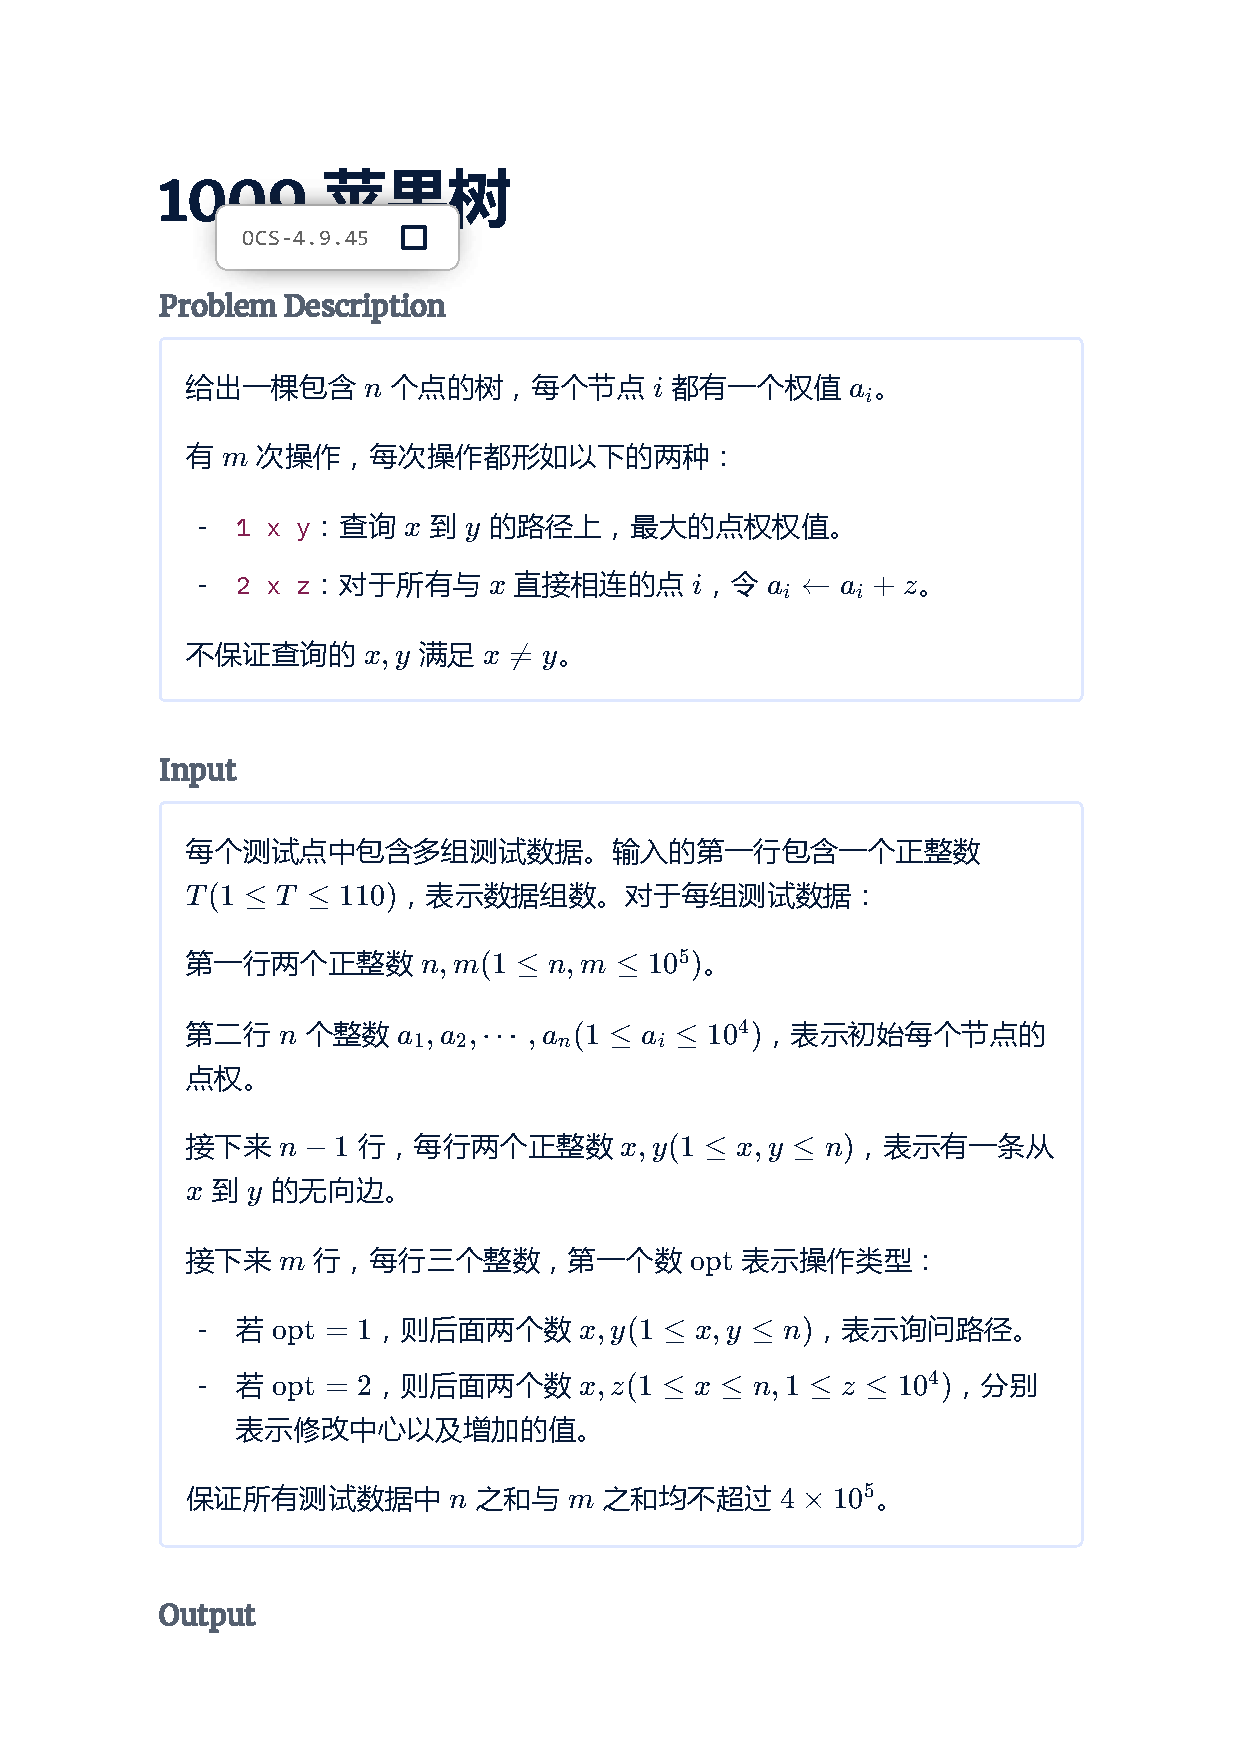
\includegraphics[page=1,width=0.94\linewidth,height=0.90\textheight,keepaspectratio]{assets/pdf/pdf_027.pdf}
\end{center}
\clearpage
\begin{center}
\includegraphics[page=2,width=0.94\linewidth,height=0.90\textheight,keepaspectratio]{assets/pdf/pdf_027.pdf}
\end{center}
\clearpage

\section{点分治}
\entrymeta{$O(n\log n)$}
\subsection{P4178 Tree}\label{p4178-tree}






\begin{codeline}
const int N = 40005;
const int K = 20005;

class Edge {
public:
    int v, w;
};

class Node {
public:
    vector<Edge> oe;
    int w;
    bool exist;
};

Node node[N];

int n;

void getW(int u, int fa) {
    node[u].w = 1;
    for(Edge& e : node[u].oe) {
        if(e.v != fa && node[e.v].exist) {
            getW(e.v, u);
            node[u].w += node[e.v].w;
        }
    }
}

int getCentroid(int u, int fa, int tot) {
    if(node[u].w * 2 < tot) {
        return 0;
    } else {
        for(Edge& e : node[u].oe) {
            if(e.v != fa && node[e.v].exist) {
                int ans = getCentroid(e.v, u, tot);
                if(ans > 0) {
                    return ans;
                }
            }
        }
        return u;
    }
}

BIT<> judge;
\end{codeline}
\vspace{-0.9\baselineskip}
\begin{codeline}[firstnumber=47]
map<int, int> tmpmem;
int k;

void dfs(int u, int fa, int d) {
    if(d <= k) {
        if(tmpmem.count(d)) {
            tmpmem[d]++;
        } else {
            tmpmem[d] = 1;
        }
    }
    node[u].w = 1;
    for(Edge& e : node[u].oe) {
        if(e.v != fa && node[e.v].exist) {
            dfs(e.v, u, d + e.w);
            node[u].w += node[e.v].w;
        }
    }
}

int main() {
    ios::sync_with_stdio(false);
    cin.tie(nullptr);
    cin >> n;
    int u, v, w;
    long long ans = 0;

    for(int i = 1; i < n; i++) {
        node[i].exist = true;
        cin >> u >> v >> w;
        node[u].oe.push_back({v, w});
        node[v].oe.push_back({u, w});
    }
    node[n].exist = true;

    cin >> k;

    getW(1, 0);
    u = getCentroid(1, 0, node[1].w);
    judge.init(k + 1);
    queue<int> que;
    que.push(u);
    while(!que.empty()) {
        u = que.front();
        que.pop();
        node[u].exist = false;
\end{codeline}
\vspace{-0.9\baselineskip}
\begin{codeline}[firstnumber=93]
        fill(judge.arr.begin(), judge.arr.end(), 0);
        judge.add(1, 1);

        for(Edge& e : node[u].oe) {
            if(node[e.v].exist) {
                tmpmem.clear();
                dfs(e.v, u, e.w);
                for(pair<int, int> p : tmpmem) {
                    ans += p.second * judge.prefix(k - p.first + 1);
                }
                for(pair<int, int> p : tmpmem) {
                    judge.add(p.first + 1, p.second);
                }
                que.push(getCentroid(e.v, u, node[e.v].w));
            }
        }
    }

    cout << (ans);
}
\end{codeline}
\begin{warnbox}
每次找重心，容斥减去同一子树内的路径。
\end{warnbox}

\section{动态重心}
\entrymeta{$O(\log n)$ 均摊}
\begin{codeline}
const int N = 100005;
int n, m;

class Data {
public:
    long long w, vw;
};

class Tag {
public:
    bool rev;
};

const Tag TAG_EP = {false};
const Tag TAG_REV = {true};

class Node {
public:
    int son[2];
    int fa;
    Data data;
    Tag tag;
    void operator+=(const Tag& t) {
        if(t.rev) {
            swap(son[0], son[1]);
            tag.rev ^= t.rev;
        }
    }
};

class LCT {
#define ls(u) (node[u].son[0])
#define rs(u) (node[u].son[1])
#define fa(u) (node[u].fa)
#define data(u) (node[u].data)
#define tag(u) (node[u].tag)
public:
    const static int MAXN = N;
    Node node[MAXN];

    bool dir(const int u) {
        return rs(fa(u)) == u;
    }

    bool is_root(const int u) {
        return ls(fa(u)) != u && rs(fa(u)) != u;
\end{codeline}
\vspace{-0.9\baselineskip}
\begin{codeline}[firstnumber=47]
    }

    void push_up(const int u) {
        data(u).w = data(ls(u)).w + data(rs(u)).w + data(u).vw + 1;
    }

    void push_down(const int u) {
        if(ls(u)) {
            node[ls(u)] += tag(u);
        }
        if(rs(u)) {
            node[rs(u)] += tag(u);
        }
        tag(u) = TAG_EP;
    }

    void update(int u) {
        if(!is_root(u)) {
            update(fa(u));
        }
        push_down(u);
    }

    void rot(int u) {
        int y = fa(u), z = fa(y), k = dir(u), v = node[u].son[!k];
        if(!is_root(y)) {
            node[z].son[dir(y)] = u;
        }
        node[y].son[k] = v;
        node[u].son[!k] = y;
        fa(v) = y;
        fa(y) = u;
        fa(u) = z;
        push_up(y);
        push_up(u);
    }

    void splay(int u) {
        update(u);
        for(int f = fa(u); !is_root(u); rot(u), f = fa(u)) {
            if(!is_root(f)) {
                rot(dir(u) == dir(f) ? f : u);
            }
        }
    }

\end{codeline}
\vspace{-0.9\baselineskip}
\begin{codeline}[firstnumber=93]
    /*
     * 打通原树根到u的实链
     */
    int access(int u) {
        int v;
        for(v = 0; u; v = u, u = fa(u)) {
            splay(u);
            data(u).vw += data(rs(u)).w - data(v).w;
            rs(u) = v;
            push_up(u);
        }
        return v;
    }

    /*
     * 将u设为所在原树的根
     */
    void make_root(int u) {
        access(u);
        splay(u);
        node[u] += TAG_REV;
    }

    /*
     * 返回u所在原树的根
     */
    int find_root(int u) {
        access(u);
        splay(u);
        push_down(u);
        while(ls(u)) {
            u = ls(u);
            push_down(u);
        }
        splay(u);
        return u;
    }

    /*
     * 将x到y的路径暴露到以y为根的辅助树，x、y须连通
     */
    void split(int x, int y) {
        make_root(x);
        access(y);
        splay(y);
    }
\end{codeline}
\vspace{-0.9\baselineskip}
\begin{codeline}[firstnumber=139]

    /*
     * 连接x、y；只在两点不连通时加边
     */
    void link(int x, int y) {
        make_root(x);
        if(find_root(y) != x) {
            splay(y);
            fa(x) = y;
            data(y).vw += data(x).w;
            push_up(y);
        }
    }

    /*
     * 断开x、y之间的直接边
     */
    void cut(int x, int y) {
        make_root(x);
        if(find_root(y) == x && fa(y) == x && !ls(y)) {
            fa(y) = rs(x) = 0;
            push_up(x);
        }
    }

    /*
     * 沿维护的权值寻找重心候选
     */
    int find_w(int u) {
        long long lw = 0, fw = 0;
        long long tot = data(u).w;
        int lans = 0, rans = 0;
        while(u) {
            push_down(u);
            int ow = data(u).w - data(rs(u)).w;
            if((fw + ow) * 2 <= tot) {
                fw += ow;
                lans = u;
                lw = fw;
                u = rs(u);
            } else {
                rans = u;
                u = ls(u);
            }
        }

\end{codeline}
\vspace{-0.9\baselineskip}
\begin{codeline}[firstnumber=185]
        if(lw == tot - lw) {
            return min(lans, rans);
        } else if(lw < tot - lw) {
            return rans;
        } else {
            return lans;
        }
    }
#undef ls
#undef rs
#undef fa
#undef data
#undef tag
};

LCT lct;
DSU dsu;
int capi[N];
char op[128];

int main() {
    ios::sync_with_stdio(false);
    cin.tie(nullptr);
    cin >> n >> m;
    dsu.init(n);
    int ans = 0;
    for(int i = 1; i <= n; i++) {
        lct.node[i].data.w = 1;
        capi[i] = i;
        ans ^= i;
    }
    int x, y;
    while(m--) {
        cin >> (op);
        if(op[0] == 'A') {
            cin >> x >> y;
            int cx = capi[dsu.find(x)];
            int cy = capi[dsu.find(y)];
            lct.link(x, y);
            lct.split(cx, cy);
            int cn = lct.find_w(cy);
            lct.splay(cn);
            ans ^= cx;
            ans ^= cy;
            ans ^= cn;
            dsu.join(x, y);
\end{codeline}
\vspace{-0.9\baselineskip}
\begin{codeline}[firstnumber=231]
            capi[dsu.find(x)] = cn;
        } else if(op[0] == 'Q') {
            cin >> x;
            cout << (capi[dsu.find(x)]) << '\n';
        } else {
            cout << (ans) << '\n';
        }
    }
}
\end{codeline}
\begin{warnbox}
LCT 维护虚子树大小；答案在路径上二分。
\end{warnbox}

\section{虚树}
\entrymeta{$O(k\log k)$}
\subsection{P2495 {[}SDOI2011{]} 消耗战 /【模板】虚树}\label{p2495-sdoi2011-ux6d88ux8017ux6218-ux6a21ux677fux865aux6811}






\begin{codeline}
const int N = 250005;
const int LOGN = 19;
const int64 INF = 0x3f3f3f3f3f3f3f3f;
int n, m;
class Edge {
public:
    int v, w;
};

class Node {
public:
    vector<Edge> oe;
    int fa[LOGN], mini[LOGN];
    int d, dfn;
};

Node node[N];

class VNode {
public:
    vector<Edge> oe;
    bool critical;
    int c;
    int64 dp;
};

VNode vnode[N];

int dfncnt = 1;

void build(int u, int fa, int d) {
    node[u].d = d;
    node[u].fa[0] = fa;
    node[u].dfn = dfncnt++;
    for(Edge& e : node[u].oe) {
        if(e.v != fa) {
            node[e.v].mini[0] = e.w;
            build(e.v, u, d + 1);
        }
    }
}

int a[N * 2];
int h[N];

bool cmp(const int A, const int B) {
\end{codeline}
\vspace{-0.9\baselineskip}
\begin{codeline}[firstnumber=47]
    return node[A].dfn < node[B].dfn;
}

void update(int u, int c) {
    if(vnode[u].c != c) {
        vnode[u].oe.clear();
        vnode[u].dp = INF;
        vnode[u].c = c;
        vnode[u].critical = false;
    }
}

/*
 * 在虚树上合并子树信息
 */
void dfs(int u) {
    int64 sum = 0;
    for(Edge& e : vnode[u].oe) {
        vnode[e.v].dp = e.w;
        dfs(e.v);
        sum += vnode[e.v].dp;
    }
    if(!vnode[u].critical) {
        vnode[u].dp = min(vnode[u].dp, sum);
    }
}

/*
 * 返回u、v的最近公共祖先，需先建好倍增表
 */
int getLCA(int u, int v) {
    if(node[u].d < node[v].d) {
        swap(u, v);
    }
    for(int j = LOGN - 1; j >= 0; j--) {
        if(node[u].d - (1 << j) >= node[v].d) {
            u = node[u].fa[j];
        }
    }
    if(u == v) {
        return u;
    }
    for(int j = LOGN - 1; j >= 0; j--) {
        if(node[u].fa[j] != node[v].fa[j]) {
            u = node[u].fa[j];
            v = node[v].fa[j];
\end{codeline}
\vspace{-0.9\baselineskip}
\begin{codeline}[firstnumber=93]
        }
    }
    return node[u].fa[0];
}

int main() {
    ios::sync_with_stdio(false);
    cin.tie(nullptr);
    int u, v, w;
    cin >> n;
    for(int i = 1; i < n; i++) {
        cin >> u >> v >> w;
        node[u].oe.push_back({v, w});
        node[v].oe.push_back({u, w});
    }

    build(1, 0, 1);

    for(int i = 1; i < LOGN; i++) {
        for(int j = 1; j <= n; j++) {
            node[j].fa[i] = node[node[j].fa[i - 1]].fa[i - 1];
            node[j].mini[i] = min(node[j].mini[i - 1], node[node[j].fa[i - 1]].mini[i - 1]);
        }
    }

    cin >> m;
    for(int T = 1; T <= m; T++) {
        int k;
        cin >> k;
        for(int i = 1; i <= k; i++) {
            cin >> h[i];
        }
        sort(h + 1, h + 1 + k, cmp);

        int l = 0;
        a[++l] = 1;
        for(int i = 1; i < k; i++) {
            a[++l] = h[i];
            a[++l] = getLCA(h[i], h[i + 1]);
        }
        a[++l] = h[k];

        sort(a + 1, a + 1 + l, cmp);
        l = unique(a + 1, a + 1 + l) - (a + 1);

        for(int i = 1; i < l; i++) {
\end{codeline}
\vspace{-0.9\baselineskip}
\begin{codeline}[firstnumber=139]
            w = 0x3f3f3f3f;
            int lca = getLCA(a[i], a[i + 1]);
            int x = a[i + 1];
            for(int j = LOGN - 1; j >= 0; j--) {
                if(node[x].d - (1 << j) >= node[lca].d) {
                    w = min(w, node[x].mini[j]);
                    x = node[x].fa[j];
                }
            }
            update(lca, T);
            update(a[i + 1], T);
            vnode[lca].oe.push_back({a[i + 1], w});
        }

        for(int i = 1; i <= k; i++) {
            vnode[h[i]].critical = true;
        }

        vnode[1].dp = INF;
        dfs(1);

        cout << (vnode[1].dp) << '\n';
    }
    return 0;
}
\end{codeline}
\begin{warnbox}
\texttt{LOGN} 按 n 取；建虚树前按 dfn 排序并加入相邻点 LCA。
\end{warnbox}

\section{基环树}
\entrymeta{$O(n)$}
\subsection{P7752 {[}COCI 2013/2014 \#2{]} PALETA}\label{p7752-coci-20132014-2-paleta}






\begin{codeline}
const int N = 1000005;
const long long MODER = 1000000007;
class Node {
public:
    int sub;
    int ptr;
    int dfn_or_ie;
    bool on_loop;
    bool visited;
};
Node node[N];
int n, k;
int dfn = 1;
int begin_dfn;
int loop_root_dfn;

long long int mul(int a, int b) {
    long long temp = a;
    temp *= (long long)b;
    temp %= MODER;
    return temp;
}

/*
 * 从idx寻找基环并记录环上节点
 */
inline void findLoop(int idx) {
    stack<int> s;

    while(!s.empty()) {
        node[idx].dfn_or_ie = dfn;
        dfn++;

        int v = node[idx].ptr;
        if(node[v].dfn_or_ie >= begin_dfn) {
            loop_root_dfn = node[v].dfn_or_ie;
        }
        if(!loop_root_dfn && !node[v].dfn_or_ie) {
            s.push(v);
        } else {
            s.pop();
        }
    }

    while(!s.empty()) {
        if(loop_root_dfn && node[idx].dfn_or_ie >= loop_root_dfn) {
\end{codeline}
\vspace{-0.9\baselineskip}
\begin{codeline}[firstnumber=47]
            node[idx].on_loop = true;
        }
    }
}

int main() {
    ios::sync_with_stdio(false);
    cin.tie(nullptr);
    cin >> n >> k;
    int num;
    for(int i = 1; i <= n; i++) {
        cin >> num;
        node[i].ptr = num;
    }
    long long ans = 1;
    for(int i = 1; i <= n; i++) {
        if(!node[i].dfn_or_ie) {
            begin_dfn = dfn;
            loop_root_dfn = 0;
            findLoop(i);
        }
    }

    for(int i = 1; i <= n; i++) {
        node[i].dfn_or_ie = 0;
        node[i].sub = 1;
    }

    for(int i = 1; i <= n; i++) {
        node[node[i].ptr].dfn_or_ie++;
    }

    int cur;
    for(int i = 1; i <= n; i++) {
        cur = i;
        while(!node[cur].dfn_or_ie && !node[cur].visited) {
            node[cur].visited = true;
            if(!node[cur].on_loop) {
                node[cur].sub = mul(node[cur].sub, k - 1);
            }
            node[node[cur].ptr].sub = mul(node[node[cur].ptr].sub, node[cur].sub);
            node[node[cur].ptr].dfn_or_ie--;
            cur = node[cur].ptr;
        }
    }

\end{codeline}
\vspace{-0.9\baselineskip}
\begin{codeline}[firstnumber=93]
    for(int i = 1; i <= n; i++) {
        if(!node[i].visited) {
            node[i].visited = true;
            int res = node[i].sub;
            int on_loop_cnt;
            int start = node[i].ptr;

            if(start == i) {
                on_loop_cnt = k;
            } else {
                int e_cnt = 1;
                on_loop_cnt = k - 1;
                for(int j = start; j != i; j = node[j].ptr) {
                    e_cnt++;
                    node[j].visited = true;
                    on_loop_cnt = mul(on_loop_cnt, (k - 1)) % MODER;
                    res = mul(res, node[j].sub) % MODER;
                }
                if(e_cnt % 2) {
                    on_loop_cnt = ((long long)on_loop_cnt + MODER - k + 1) % MODER;
                } else {
                    on_loop_cnt = ((long long)on_loop_cnt + k - 1) % MODER;
                }
            }
            ans = ans * res % MODER * on_loop_cnt % MODER;
        }
    }

    cout << (ans) << '\n';
}
\end{codeline}
\begin{warnbox}
先找环，再对环上每棵树 DP，最后环上断边处理。
\end{warnbox}


\chapter{网络流}

\section{最大流}
\entrymeta{ISAP $O(n^2m)$；HLPP $O(n^2\sqrt m)$}
调用前提：先 init(n)，节点编号在 1..n 内，容量非负，源汇不同。


\begin{codeline}
class ISAP {
public:
    class Edge {
    public:
        int v;
        int64 c;
    };
    class Node {
    public:
        vector<int> oe;
        int d = 0, ce = 0, pre = 0;
    };
    vector<Edge> edge;
    vector<Node> node;
    vector<int> gap;
    int cnt = 0, src = 0, terminal = 0;

    /*
     * 初始化 n 个点的残量网络
     */
    void init(int n) {
        cnt = n;
        node.assign(n + 1, Node());
        gap.assign(n + 1, 0);
        edge.clear();
        src = terminal = 0;
    }

    /*
     * 添加 u 到 v、容量为 c 的边及其反向边
     */
    void add_edge(int u, int v, int64 c) {
        int id = int(edge.size());
        node[u].oe.push_back(id);
        node[v].oe.push_back(id + 1);
        edge.push_back({v, c});
        edge.push_back({u, 0});
    }

    /*
     * 从汇点反向 BFS，求各点到汇点的最短距离并统计 gap
     */
    void get_level_graph() {
        for(auto& u : node) {
            u.d = cnt;
            u.ce = 0;
\end{codeline}
\vspace{-0.9\baselineskip}
\begin{codeline}[firstnumber=47]
            u.pre = 0;
        }
        fill(gap.begin(), gap.end(), 0);
        queue<int> q;
        q.push(terminal);
        node[terminal].d = 0;
        gap[0] = 1;
        while(!q.empty()) {
            int u = q.front();
            q.pop();
            for(int id : node[u].oe) {
                int v = edge[id].v;
                if(edge[id ^ 1].c && node[v].d == cnt) {
                    node[v].d = node[u].d + 1;
                    gap[node[v].d]++;
                    q.push(v);
                }
            }
        }
    }

    /*
     * 沿 pre 从汇点回溯到源点，增广并返回本次流量
     */
    int64 augment() {
        int64 f = numeric_limits<int64>::max();
        for(int u = terminal; u != src; u = edge[node[u].pre ^ 1].v) {
            f = min(f, edge[node[u].pre].c);
        }
        for(int u = terminal; u != src; u = edge[node[u].pre ^ 1].v) {
            edge[node[u].pre].c -= f;
            edge[node[u].pre ^ 1].c += f;
        }
        return f;
    }

    /*
     * 求 s 到 t 的最大流，修改残量网络
     */
    int64 max_flow(int s, int t) {
        src = s;
        terminal = t;
        get_level_graph();
        int64 ans = 0;
        int u = src;
        while(node[src].d < cnt) {
\end{codeline}
\vspace{-0.9\baselineskip}
\begin{codeline}[firstnumber=93]
            if(u == terminal) {
                ans += augment();
                u = src;
                continue;
            }
            bool found = false;
            for(int& i = node[u].ce; i < int(node[u].oe.size()); i++) {
                int id = node[u].oe[i];
                if(edge[id].c && node[u].d == node[edge[id].v].d + 1) {
                    node[edge[id].v].pre = id;
                    found = true;
                    u = edge[id].v;
                    break;
                }
            }
            if(found) {
                continue;
            }
            int min_d = cnt - 1;
            for(int id : node[u].oe) {
                if(edge[id].c && node[edge[id].v].d < min_d) {
                    min_d = node[edge[id].v].d;
                }
            }
            gap[node[u].d]--;
            if(gap[node[u].d] == 0) {
                break;
            }
            node[u].d = min_d + 1;
            gap[node[u].d]++;
            node[u].ce = 0;
            if(u != src) {
                u = edge[node[u].pre ^ 1].v;
            }
        }
        return ans;
    }
};
\end{codeline}
\begin{codeline}
constexpr int N = 1200, M = 120000, INF = 0x3f3f3f3f;
int n, m, s, t;

struct qxx {
    int nex, t;
    long long v;
};

qxx e[M * 2 + 1];
int h[N + 1], cnt = 1;

void add_path(int f, int t, long long v) {
    e[++cnt] = qxx{h[f], t, v};
    h[f] = cnt;
}

/*
 * 添加容量边及对应反向边
 */
void add_flow(int f, int t, long long v) {
    add_path(f, t, v);
    add_path(t, f, 0);
}

int ht[N + 1];       // 高度;
long long ex[N + 1]; // 超额流;
int gap[N];          // gap 优化. gap[i] 为高度为 i 的节点的数量
stack<int> B[N];     // 桶 B[i] 中记录所有 ht[v]==i 的v
int level = 0;       // 溢出节点的最高高度

int push(int u) {       // 尽可能通过能够推送的边推送超额流
    bool init = u == s; // 是否在初始化
    for(int i = h[u]; i; i = e[i].nex) {
        const int& v = e[i].t;
        const long long& w = e[i].v;
        // 初始化时不考虑高度差为1
        if(!w || (init == false && ht[u] != ht[v] + 1) || ht[v] == INF) {
            continue;
        }
        long long k = init ? w : min(w, ex[u]);
        // 取到剩余容量和超额流的最小值，初始化时可以使源的溢出量为负数。
        if(v != s && v != t && !ex[v]) {
            B[ht[v]].push(v);
            level = max(level, ht[v]);
        }
        ex[u] -= k, ex[v] += k, e[i].v -= k, e[i ^ 1].v += k; // push
\end{codeline}
\vspace{-0.9\baselineskip}
\begin{codeline}[firstnumber=47]
        if(!init && !ex[u]) {
            return 0; // 如果已经推送完就返回；初始化阶段源点可为负，不能提前返回
        }
    }
    return 1;
}

void relabel(int u) { // 重贴标签（高度）
    ht[u] = INF;
    for(int i = h[u]; i; i = e[i].nex) {
        if(e[i].v) {
            ht[u] = min(ht[u], ht[e[i].t]);
        }
    }
    if(++ht[u] < n) { // 只处理高度小于 n 的节点
        B[ht[u]].push(u);
        level = max(level, ht[u]);
        ++gap[ht[u]]; // 新的高度，更新 gap
    }
}

bool bfs_init() {
    memset(ht, 0x3f, sizeof(ht));
    queue<int> q;
    q.push(t);
    ht[t] = 0;
    while(q.size()) { // 反向 BFS, 遇到没有访问过的结点就入队
        int u = q.front();
        q.pop();
        for(int i = h[u]; i; i = e[i].nex) {
            const int& v = e[i].t;
            if(e[i ^ 1].v && ht[v] > ht[u] + 1) {
                ht[v] = ht[u] + 1;
                q.push(v);
            }
        }
    }
    return ht[s] != INF; // 如果图不连通，返回 0
}

// 选出当前高度最大的节点之一, 如果已经没有溢出节点返回 0
int select() {
    while(level > -1 && B[level].size() == 0) {
        level--;
    }
    return level == -1 ? 0 : B[level].top();
\end{codeline}
\vspace{-0.9\baselineskip}
\begin{codeline}[firstnumber=93]
}

long long hlpp() { // 返回最大流
    if(!bfs_init()) {
        return 0; // 图不连通
    }
    memset(gap, 0, sizeof(gap));
    for(int i = 1; i <= n; i++) {
        if(ht[i] != INF) {
            gap[ht[i]]++; // 初始化 gap
        }
    }
    ht[s] = n;
    push(s); // 初始化预流
    int u;
    while((u = select())) {
        B[level].pop();
        if(push(u)) { // 仍然溢出
            if(!--gap[ht[u]]) {
                for(int i = 1; i <= n; i++) {
                    if(i != s && ht[i] > ht[u] && ht[i] < n + 1) {
                        ht[i] = n + 1; // 这里重贴成 n+1 的节点都不是溢出节点
                    }
                }
            }
            relabel(u);
        }
    }
    return ex[t];
}

int main() {
    ios::sync_with_stdio(false);
    cin.tie(nullptr);
    cin >> n >> m >> s >> t;
    for(int i = 1, u, v, w; i <= m; i++) {
        cin >> u >> v >> w;
        add_flow(u, v, w);
    }
    cout << (hlpp());
    return 0;
}
\end{codeline}
\begin{warnbox}
ISAP 用 \texttt{d = cnt} 作哨兵；HLPP 初始化阶段源点超额可为负，不能提前返回。
\end{warnbox}

\section{费用流}
\entrymeta{$O(Fm\log n)$}
\subsection{P3381 【模板】最小费用最大流}\label{p3381-ux6a21ux677fux6700ux5c0fux8d39ux7528ux6700ux5927ux6d41}


\begin{codeline}
const int64 MAXN = 5005;
const int64 INF = 0x3f3f3f3f3f3f3f3f;

struct Edge {
    int64 v, cost, capacity, flow;
};

class Node {
public:
    vector<int64> level_oe;
    int64 cur_edge;
    int64 dis;
    int64 h;
    bool visited;
};

class State {
public:
    int64 u, cost;
};

bool operator<(const State& A, const State& B) {
    return A.cost > B.cost;
}

class PrimalDual {
public:
    int64 node_cnt;
    int64 edge_cnt;
    int64 src, terminal;
    int64 tot_flow;
    int64 tot_cost;
    vector<Edge> edges;
    Node node[MAXN];

    /*
     * 添加容量为capacity、单位费用为cost的有向边
     */
    void add_edge(int64 u, int64 v, int64 capacity, int64 cost) {
        node[u].level_oe.push_back(edge_cnt++);
        node[v].level_oe.push_back(edge_cnt++);
        edges.push_back({v, cost, capacity, 0});
        edges.push_back({u, -cost, 0, 0});
    }

    void SPFA() {
\end{codeline}
\vspace{-0.9\baselineskip}
\begin{codeline}[firstnumber=47]
        queue<int64> q;
        q.push(src);
        node[src].visited = true;

        int64 u;
        while(!q.empty()) {
            u = q.front();
            q.pop();
            node[u].visited = false;
            for(int64 i = 0; i < node[u].level_oe.size(); i++) {
                Edge& e = edges[node[u].level_oe[i]];
                if(e.capacity > e.flow && node[e.v].h > node[u].h + e.cost) {
                    node[e.v].h = node[u].h + e.cost;
                    if(!node[e.v].visited) {
                        q.push(e.v);
                        node[e.v].visited = true;
                    }
                }
            }
        }
    }

    bool dijkstra() {
        for(int i = 0; i <= node_cnt; i++) {
            node[i].cur_edge = 0;
            node[i].dis = INF;
            node[i].visited = false;
        }

        priority_queue<State> q;
        q.push({src, 0});
        node[src].dis = 0;

        int64 u;
        int64 l;
        State tmp;
        while(!q.empty()) {
            tmp = q.top();
            u = tmp.u;
            q.pop();
            if(node[u].visited) {
                continue;
            } else {
                node[u].visited = true;
            }
            for(int64 i = 0; i < node[u].level_oe.size(); i++) {
\end{codeline}
\vspace{-0.9\baselineskip}
\begin{codeline}[firstnumber=93]
                Edge& e = edges[node[u].level_oe[i]];
                l = e.cost + node[u].h - node[e.v].h;
                if(e.capacity > e.flow && node[e.v].dis > node[u].dis + l) {
                    node[e.v].dis = node[u].dis + l;
                    q.push({e.v, node[e.v].dis});
                }
            }
        }
        return node[terminal].dis != INF;
    }

    /*
     * 清空残量网络并设置点数
     */
    void init(int64 cnt) {
        node_cnt = cnt;
        edge_cnt = 0;
        for(int64 i = 0; i <= node_cnt; i++) {
            node[i] = Node();
        }
        edges.clear();
    }

    int64 augment(int64 v, int64 flow) {
        if(v == src) {
            return flow;
        }

        node[v].visited = true;
        int64 res;
        int64 ans = 0;
        int64 u, l;
        for(int64& i = node[v].cur_edge; i < node[v].level_oe.size(); i++) {
            Edge& come_e = edges[node[v].level_oe[i] ^ 1];
            Edge& back_e = edges[node[v].level_oe[i]];
            u = back_e.v;
            l = come_e.cost + node[u].h - node[v].h;

            if((!node[u].visited) && node[v].dis == node[u].dis + l && come_e.capacity > come_e.flow) {
                res = augment(u, min(come_e.capacity - come_e.flow, flow));
                ans += res;
                back_e.flow -= res;
                come_e.flow += res;
                flow -= res;
                if(!flow) {
                    break;
\end{codeline}
\vspace{-0.9\baselineskip}
\begin{codeline}[firstnumber=139]
                }
            }
        }
        node[v].visited = false;
        return ans;
    }

    /*
     * 求s到t的最小费用最大流，结果保存在tot_flow和tot_cost
     */
    void calc(int64 s, int64 t) {
        src = s;
        terminal = t;
        tot_cost = 0;
        tot_flow = 0;
        for(int i = 0; i <= node_cnt; i++) {
            node[i].h = INF;
        }
        node[src].h = 0;
        SPFA(); // 第一轮依旧得 SPFA

        for(int i = 0; i <= node_cnt; i++) {
            if(node[i].h == INF) {
                node[i].h = 0;
            }
        }
        int64 flow;
        while(dijkstra()) { // 后面用Dji
            for(int i = 0; i <= node_cnt; i++) {
                node[i].visited = false;
            }

            flow = augment(terminal, INF);

            for(int i = 0; i <= node_cnt; i++) {
                if(node[i].dis != INF) {
                    node[i].h += node[i].dis;
                }
            }

            tot_flow += flow;
            tot_cost += flow * node[terminal].h;
        }
    }
};

\end{codeline}
\vspace{-0.9\baselineskip}
\begin{codeline}[firstnumber=185]
PrimalDual primalDual;
\end{codeline}


\subsection{P4843 清理雪道}\label{p4843-ux6e05ux7406ux96eaux9053}


\begin{codeline}
/*
 * 本题边权为 1，路径费用只会是 0 或 -1。
 * PrimalDual 的其余成员直接继承，只覆盖 calc：最短路径费用非负时停止增广。
 */
class SnowFlow : public PrimalDual {
public:
    /* 其余方法继承自 PrimalDual，不重复抄写 */
    void calc(int64 s, int64 t, int64 stop) {
        src = s;
        terminal = t;
        tot_cost = 0;
        tot_flow = 0;
        for(int i = 0; i <= node_cnt; i++) {
            node[i].h = INF;
        }
        node[src].h = 0;
        SPFA();
        for(int i = 0; i <= node_cnt; i++) {
            if(node[i].h == INF) {
                node[i].h = 0;
            }
        }
        int64 flow;
        while(dijkstra()) {
            if(node[terminal].h + node[terminal].dis >= stop) {
                break;
            }
            for(int i = 0; i <= node_cnt; i++) {
                node[i].visited = false;
            }
            flow = augment(terminal, INF);
            for(int i = 0; i <= node_cnt; i++) {
                if(node[i].dis != INF) {
                    node[i].h += node[i].dis;
                }
            }
            tot_flow += flow;
            tot_cost += flow * node[terminal].h;
        }
    }
};

SnowFlow snowFlow;

int64 ie[MAXN], oe[MAXN];

\end{codeline}
\vspace{-0.9\baselineskip}
\begin{codeline}[firstnumber=47]
int main() {
    ios::sync_with_stdio(false);
    cin.tie(nullptr);
    int64 n, m;

    cin >> n;
    snowFlow.init(n + 2);
    int64 v;
    for(int64 i = 1; i <= n; i++) {
        cin >> m;
        oe[i] = m;
        for(int64 j = 0; j < m; j++) {
            cin >> v;
            ie[v]++;
            snowFlow.add_edge(i, v, 1, -1);
            snowFlow.add_edge(i, v, INF, 0);
        }
    }

    for(int64 i = 1; i <= n; i++) {
        if(!ie[i]) {
            snowFlow.add_edge(n + 1, i, INF, 0);
        }
        if(!oe[i]) {
            snowFlow.add_edge(i, n + 2, INF, 0);
        }
    }

    snowFlow.calc(n + 1, n + 2, 0);
    cout << (snowFlow.tot_flow) << '\n';
}
\end{codeline}
\begin{warnbox}
先 SPFA 求初始势能，之后 Dijkstra；负费用边需保证无负环。
\end{warnbox}


\chapter{连通性}

\section{割点}
\entrymeta{$O(n+m)$}
\subsection{P3388 【模板】割点（割顶）}\label{p3388-ux6a21ux677fux5272ux70b9ux5272ux9876}


\begin{codeline}
#define N 20005
int n, m;
vector<int> oe[N];
bool visited[N];
bool isCutVertex[N];
int dfn[N];
int low[N];
int cnt = 0;
/*
 * 维护dfn、low并标记割点，fa为DFS树父节点
 */
void tarjan(int idx, int fa) {
    cnt++;
    visited[idx] = true;
    low[idx] = dfn[idx] = cnt;
    int child = 0;
    for(int e : oe[idx]) {
        if(!visited[e]) {
            child++;
            tarjan(e, idx);
            low[idx] = min(low[idx], low[e]);
            if(fa != 0 && low[e] >= dfn[idx]) {
                isCutVertex[idx] = true;
            }
        } else if(e != fa) {
            low[idx] = min(low[idx], dfn[e]);
        }
    }
    if(fa == 0 && child >= 2) {
        isCutVertex[idx] = true;
    }
}
int main() {
    ios::sync_with_stdio(false);
    cin.tie(nullptr);
    cin >> n >> m;
    int u, v;
    while(m-- > 0) {
        cin >> u >> v;
        oe[u].push_back(v);
        oe[v].push_back(u);
    }

    for(int i = 1; i <= n; i++) {
        if(!visited[i]) {
            tarjan(i, 0);
\end{codeline}
\vspace{-0.9\baselineskip}
\begin{codeline}[firstnumber=47]
        }
    }

    int res = 0;
    for(int i = 1; i <= n; i++) {
        res += isCutVertex[i];
    }
    cout << (res) << '\n';

    for(int i = 1; i <= n; i++) {
        if(isCutVertex[i]) {
            cout << (i) << ' ';
        }
    }
}
\end{codeline}
\begin{warnbox}
\texttt{low[v] \textgreater{}= dfn[u]} 判割点；根需单独统计儿子数。
\end{warnbox}

\section{缩点}
\entrymeta{$O(n+m)$}
\subsection{P3387 【模板】缩点}\label{p3387-ux6a21ux677fux7f29ux70b9}


\begin{codeline}
const int N = 10005;

class SCCNode {
public:
    vector<int> oe;
    int dfn, low;
    int color;
    int ie;
    int w;
    bool inStack;
};

vector<int> st;

class Node {
public:
    vector<int> oe;
    int sum;
    int ie;
    int dp;
};

SCCNode scc[N];
Node node[N];
int dfncnt = 1;

int n, m;

/*
 * 求u可达部分的强连通分量并记录分量编号
 */
void tarjan(int u) {
    scc[u].dfn = scc[u].low = dfncnt++;
    scc[u].color = u;
    st.push_back(u);
    scc[u].inStack = true;
    for(int v : scc[u].oe) {
        if(!scc[v].dfn) {
            tarjan(v);
        }
        if(scc[v].low < scc[u].low && scc[v].inStack) {
            scc[u].low = scc[v].low;
        }
    }

    if(scc[u].low == scc[u].dfn) {
\end{codeline}
\vspace{-0.9\baselineskip}
\begin{codeline}[firstnumber=47]
        int v = st.back();
        while(v != u) {
            scc[v].color = u;
            st.pop_back();
            scc[v].inStack = false;
            v = st.back();
        }
        st.pop_back();
        scc[u].inStack = false;
    }
}

int main() {
    ios::sync_with_stdio(false);
    cin.tie(nullptr);
    cin >> n >> m;
    for(int i = 1; i <= n; i++) {
        cin >> scc[i].w;
    }

    int u, v;
    for(int i = 1; i <= m; i++) {
        cin >> u >> v;
        scc[u].oe.push_back(v);
        scc[v].ie++;
    }

    for(int i = 1; i <= n; i++) {
        scc[0].oe.push_back(i);
    }

    tarjan(0);

    for(u = 1; u <= n; u++) {
        int nu = scc[u].color;
        node[nu].sum += scc[u].w;
        for(int e : scc[u].oe) {
            v = e;
            int nv = scc[v].color;
            if(nu != nv) {
                node[nu].oe.push_back(nv);
                node[nv].ie++;
            }
        }
    }

\end{codeline}
\vspace{-0.9\baselineskip}
\begin{codeline}[firstnumber=93]
    queue<int> q;
    for(u = 1; u <= n; u++) {
        if(!node[u].ie) {
            q.push(u);
        }
    }

    int ans = 0;
    while(!q.empty()) {
        u = q.front();
        q.pop();
        node[u].dp += node[u].sum;
        ans = max(ans, node[u].dp);
        for(int e : node[u].oe) {
            v = e;
            node[v].dp = max(node[v].dp, node[u].dp);
            node[v].ie--;
            if(!node[v].ie) {
                q.push(v);
            }
        }
    }

    cout << (ans);
}
\end{codeline}
\begin{warnbox}
Tarjan 后按 SCC 编号建 DAG；重复边要去重。
\end{warnbox}


\chapter{图匹配}

\section{匈牙利算法}
\entrymeta{$O(nm)$}
\subsection{P3386 【模板】二分图最大匹配}\label{p3386-ux6a21ux677fux4e8cux5206ux56feux6700ux5927ux5339ux914d}


\begin{codeline}
const int N = 505;

int n, m, e;

vector<int> edge[N];
int match[N];
int dfn[N];

/*
 * 从u寻找增广路，tag用于标记本轮访问
 */
int dfs(int u, int tag) {
    if(dfn[u] == tag) {
        return 0;
    } else {
        dfn[u] = tag;
        for(int v : edge[u]) {
            if(match[v] == 0 || dfs(match[v], tag)) {
                match[v] = u;
                return 1;
            }
        }
        return 0;
    }
}

int main() {
    ios::sync_with_stdio(false);
    cin.tie(nullptr);
    cin >> n >> m >> e;

    int u, v;
    for(int i = 0; i < e; i++) {
        cin >> u >> v;
        edge[u].push_back(v);
    }
    int ans = 0;
    for(int i = 1; i <= n; i++) {
        ans += dfs(i, i);
    }

    cout << (ans) << '\n';
}
\end{codeline}
\begin{warnbox}
每次增广前清空 \texttt{vis}。
\end{warnbox}

\section{带花树算法}
\entrymeta{$O(n^3)$}
\begin{codeline}
const int N = 1005;
int m, n, cnt;
queue<int> q;

class Node {
public:
    vector<int> oe;
    int pre;
    int match;
    int check;
    int color;
    int fa;
    int on_flower;
};

Node node[N];

int find_root(int u) {
    bool flag = false;
    int last;
    while(node[u].fa != u) {
        if(flag) {
            node[last].fa = node[u].fa;
        }
        last = u;
        u = node[u].fa;
        flag = !flag;
    }
    return u;
}

void cat(int u, int v) {
    u = find_root(u);
    v = find_root(v);
    if(u != v) {
        node[u].fa = v;
        // This is a special parallel set whose root must be the flower root.
        // Merging by rank does not apply.
    }
}

int lca(int u, int v) {
    cnt++;
    u = find_root(u);
    v = find_root(v);
    while(node[u].on_flower != cnt) {
\end{codeline}
\vspace{-0.9\baselineskip}
\begin{codeline}[firstnumber=47]
        node[u].on_flower = cnt;
        u = find_root(node[node[u].match].pre);
        if(v > 0) {
            swap(u, v);
        }
    }
    return u;
}

/*
 * 将奇环收缩到公共基点r
 */
void shrink(int u, int v, int r) {
    while(find_root(u) != find_root(r)) {
        node[u].pre = v;
        v = node[u].match;
        if(node[v].color == 1) {
            node[v].color = 0;
            q.push(v);
        }
        if(find_root(u) == u) {
            cat(u, r);
        }
        if(find_root(v) == v) {
            cat(v, r);
        }
        // These ifs are essential. Bugs always occur here.
        u = node[v].pre;
    }
}

/*
 * 为当前匹配初始化增广搜索状态
 */
void init() {
    while(!q.empty()) {
        q.pop();
    }

    for(int i = 1; i <= n; i++) {
        node[i].fa = i;
        node[i].pre = 0;
        node[i].color = -1;
    }
}

\end{codeline}
\vspace{-0.9\baselineskip}
\begin{codeline}[firstnumber=93]
/*
 * 反复寻找增广路，返回增加的匹配数
 */
int bfs() {
    int ans = 0;
    for(int i = 1; i <= n; i++) {
        if(!node[i].match) {
            init();
            q.push(i);
            node[i].color = 0;
            while(!q.empty() && !node[i].match) {
                int u = q.front();
                q.pop();
                for(int v : node[u].oe) {
                    if(node[v].color == 1 || find_root(u) == find_root(v)) {
                        continue;
                    } else if(node[v].color == 0) {
                        int root = lca(u, v);
                        shrink(u, v, root);
                        shrink(v, u, root);
                    } else {
                        node[v].color = 1;
                        node[v].pre = u;
                        if(!node[v].match) {
                            while(u > 0) {
                                int last_v = node[u].match;
                                int last_u = node[last_v].pre;
                                node[u].match = v;
                                node[v].match = u;
                                v = last_v;
                                u = last_u;
                            }
                            break;
                        } else {
                            node[node[v].match].color = 0;
                            q.push(node[v].match);
                        }
                    }
                }
            }
            if(node[i].match) {
                ans++;
            }
        }
    }
    return ans;
\end{codeline}
\vspace{-0.9\baselineskip}
\begin{codeline}[firstnumber=139]
}

int main() {
    ios::sync_with_stdio(false);
    cin.tie(nullptr);
    cin >> n >> m;
    int u, v;
    for(int i = 0; i < m; i++) {
        cin >> u >> v;
        node[u].oe.push_back(v);
        node[v].oe.push_back(u);
    }

    cout << (bfs()) << '\n';
    for(int i = 1; i <= n; i++) {
        cout << (node[i].match) << ' ';
    }
    return 0;
}
\end{codeline}
\begin{warnbox}
一般图最大匹配；缩花时注意 LCA 与并查集。
\end{warnbox}


\chapter{其他图论算法}

\section{折半搜索}
\entrymeta{$O(2^{n/2})$}
\subsection{P2962 {[}USACO09NOV{]} Lights G}\label{p2962-usaco09nov-lights-g}






\begin{codeline}
#define N 40
class Point {
public:
    vector<int> oe;
    bool state;
};

Point p[N + 1];

int n, m;
long long int a[N + 1];
map<long long, int> s;

int main() {
    ios::sync_with_stdio(false);
    cin.tie(nullptr);
    cin >> n >> m;
    int u, v;
    for(int i = 0; i < m; i++) {
        cin >> u >> v;
        p[u].oe.push_back(v);
        p[v].oe.push_back(u);
    }

    for(int i = 1; i <= n; i++) {
        long long int t = 1 << (i - 1);
        for(int j : p[i].oe) {
            t |= 1ll << (j - 1);
        }
        a[i - 1] = t;
    }

    int top = 1 << (n / 2);

    for(int i = 0; i < top; i++) {
        long long int code = 0;
        int d = 0;
        for(int j = 0; j < n / 2; j++) {
            if((i >> j) & 1) {
                code ^= a[j];
                d++;
            }
        }
        if(!s.count(code)) {
            s[code] = d;
        } else {
\end{codeline}
\vspace{-0.9\baselineskip}
\begin{codeline}[firstnumber=47]
            s[code] = min(d, s[code]);
        }
    }

    int ans = 2147483647;
    top = 1 << (n - n / 2);
    for(int i = 0; i < top; i++) {
        long long int code = 0;
        int d = 0;
        for(int j = 0; j < n - n / 2; j++) {
            if((i >> j) & 1) {
                code ^= a[n / 2 + j];
                d++;
            }
        }
        if(s.count(((1ll << n) - 1) ^ code)) {
            ans = min(ans, d + s[((1ll << n) - 1) ^ code]);
        }
    }

    cout << (ans);
}
\end{codeline}
\begin{warnbox}
两半分别枚举后排序双指针。
\end{warnbox}

\section{斯坦纳树}
\entrymeta{$O(3^k n + 2^k m\log m)$}
\subsection{P4294 {[}WC2008{]} 游览计划}\label{p4294-wc2008-ux6e38ux89c8ux8ba1ux5212}






\begin{codeline}
int dp[12][12][4096];
int w[12][12];
int zipper[12][12];
int128 arr[12][12][4096];
int n, m, k;
vector<pair<int, int>> key;

int direction[4][2] = {
    {0, 1},
    {1, 0},
    {0, -1},
    {-1, 0}};

class State {
public:
    int x, y, v;
};

bool operator<(const State& A, const State& B) {
    return A.v > B.v;
}

int128 bit = 1;

int main() {
    ios::sync_with_stdio(false);
    cin.tie(nullptr);
    cin >> n >> m;
    memset(dp, 0x3f, sizeof(dp));
    for(int i = 1; i <= n; i++) {
        for(int j = 1; j <= m; j++) {
            cin >> w[i][j];
            zipper[i][j] = (i - 1) * m + j - 1;
            if(!w[i][j]) {
                key.push_back({i, j});
                dp[i][j][1 << k] = 0;
                arr[i][j][1 << k] = bit << zipper[i][j];
                k++;
            }
        }
    }

    for(int s = 1; s < 1 << k; s++) {
        priority_queue<State> q;
        for(int i = 1; i <= n; i++) {
            for(int j = 1; j <= m; j++) {
\end{codeline}
\vspace{-0.9\baselineskip}
\begin{codeline}[firstnumber=47]
                for(int sub = s & (s - 1); sub; sub = s & (sub - 1)) {
                    if(dp[i][j][s] > dp[i][j][sub] + dp[i][j][s ^ sub] - w[i][j]) {
                        dp[i][j][s] = dp[i][j][sub] + dp[i][j][s ^ sub] - w[i][j];
                        arr[i][j][s] = arr[i][j][sub] | arr[i][j][s ^ sub];
                    }
                }
                if(dp[i][j][s] != 0x3f3f3f3f) {
                    q.push({i, j, dp[i][j][s]});
                }
            }
        }

        while(!q.empty()) {
            State cur = q.top();
            q.pop();
            if(cur.v == dp[cur.x][cur.y][s]) {
                for(int facing = 0; facing < 4; facing++) {
                    int nxtx = cur.x + direction[facing][0];
                    int nxty = cur.y + direction[facing][1];
                    if(nxtx > 0 && nxtx <= n && nxty > 0 && nxty <= m) {
                        if(dp[nxtx][nxty][s] > dp[cur.x][cur.y][s] + w[nxtx][nxty]) {
                            dp[nxtx][nxty][s] = dp[cur.x][cur.y][s] + w[nxtx][nxty];
                            arr[nxtx][nxty][s] = arr[cur.x][cur.y][s] | (bit << zipper[nxtx][nxty]);
                            q.push({nxtx, nxty, dp[nxtx][nxty][s]});
                        }
                    }
                }
            }
        }
    }

    if(k > 0) {
        cout << (dp[key[0].first][key[0].second][(1 << k) - 1]) << '\n';
        for(int i = 1; i <= n; i++) {
            for(int j = 1; j <= m; j++) {
                if(!w[i][j]) {
                    cout << "x";
                } else {
                    int128 arrange = arr[key[0].first][key[0].second][(1 << k) - 1];
                    if(arrange & (bit << zipper[i][j])) {
                        cout << "o";
                    } else {
                        cout << "_";
                    }
                }
            }
\end{codeline}
\vspace{-0.9\baselineskip}
\begin{codeline}[firstnumber=93]
            cout << '\n';
        }
    } else {
        cout << "0\n";
        for(int i = 1; i <= n; i++) {
            for(int j = 1; j <= m; j++) {
                if(!w[i][j]) {
                    cout << "x";
                } else {
                    cout << "_";
                }
            }
            cout << '\n';
        }
    }
}
\end{codeline}
\begin{warnbox}
先子集 DP，再对每个状态跑最短路。
\end{warnbox}

